\documentclass[12 pt,twoside]{article}
\usepackage{epsfig}
\usepackage{fullpage}
\usepackage[font={small,it}]{caption}


\begin {document}
\begin{center}

{\LARGE{\bf Nature of Light Experimentally Described by Poisson Statistics}}

{\large Tim Kornish}

University of Montana

September 29, 2014
\end{center}

\section{ABSTRACT}

The results of measuring the number of  photons emitted by a Light-Emitting Diode (LED) during certain time intervals. Repeated the experiment several times using an Agilent 53131A that counted the number of photons detected by a Photomultiplier Tube (PMT) that detects individual photons. Through the experiment it will be seen that the number of repetitions of data sets and samples per set will affect the standard deviation ($\sigma$). 

\section{INTRODUCTION}
Attempting to prove through experiment how the stander deviation ($\sigma$) will change in different scenarios of different sample sizes and different LED environments. Proving Poisson statistics hold in this experiment within reasonable error bounds, although no uncertainty was calculated. There will be 10 separate experiments analyzed using different analyzing process to compare what changes in the test environment changes what variable of Poisson statistics.                                              
             
\section{OBSERVATIONS AND DATA ANALYSIS}

All plots of data will be located at the end of the article with figure number corresponding to section number

For the first eight experiments the data will be collected using only one LED. The Last two will be collected using two LED's: one with a varying brightness with half of all data having a background LED off and the other half having the background LED on both with a constant brightness setting throughout  data collection trials.

\subsection{First Experiment}
The first experiment begins fairly simple with only one LED on. The first data set is gathered using a  set of 10 samples gathering data for 10 ms intervals shown in {\it Figure1}.

\subsection{Second Experiment}
With the data seeming random with such few samples from experiment one, the next step is to increase the sample size to 100 keeping the time interval at 10 ms. With more samples the mean and $\sigma$ of the data set was calculated with more precision. {\it Figure2}

\subsection{Third Experiment}

Taking 6 different data sets with 1000 samples per set with 10ms intervals. Using histograms instead of scatterplots for easier side by side comparison of distribution. {\it Figure3}

\subsection{Fourth Experiment}

Taking 6 different data sets with 1000 samples per set with 10ms intervals. Using histograms instead of scatterplots for easier side by side comparison of distribution. {\it Figure4}

\subsection{Fifth Experiment}

Taking 12 separate data sets all of 100 samples but varying sample time intervals ranging from 1ms to 2048ms per sample in steps of $2^n$ starting at n=0 and ending at n=11. Using the same sample size every time to determine if the time interval has an affect upon the standard deviation ($\sigma$). {\it Figure5}
 
\subsection{Sixth Experiment}

Taking 1 data set of 1000 samples with 1ms time intervals aiming for between 2-4 photons per sample. Finding the mean count rate and comparing this value to the theoretical Poisson Distribution. {\it Figure6}

\subsection{Seventh Experiment}

A second set of 1000 samples with 1ms time intervals now getting around 50 photon counts as the mean. In this case the Gaussian Curve provides a good approximation to the Poisson Distribution. {\it Figure7}

\subsection{Eighth Experiment}

Now Using the same arbitrary chosen time interval with different sample sized to show how the mean of means and $\sigma$ changes. Using sample sizes ranging from 2 to 2048 in step sizes of $2^n$ with n=1 to n=11. Then calculating the individual Standard deviation of the means $\sigma_\mu$ = $\frac{\sigma}{\sqrt{samples}}$. As seen the mean comes to an equilibrium point as the number of samples increase approximately 5.1.  {\it Figure8} 

\subsection{Ninth Experiment}

One test of 10 data sets with 20 samples and 100 ms time intervals. The samples will be divided into two groups with the first half having a background LED on and the second half having the background LED off. Performed with the background LED at a constant brightness setting and the second LED at a low brightness setting giving off very few photons in the time interval. {\it Figure9}

\subsection{Tenth Experiment}

10 data sets with 20 samples and 100 ms time intervals. The samples will be divided into two groups with the first half having a background LED on and the second half having the background LED off. Performed with the background LED at a constant brightness setting and the second LED at an initial low brightness setting giving off very few photons in the time interval ranging to a very high brightness setting to see an obvious difference between background LED begin ON vs. OFF. {\it Figure10}

\section{CONCLUSION}

Through various experiments counting photons under different environmental conditions it has been shown that certain changes will cause different $\sigma$ while other changes will have no effect. Increasing the number of samples gave more precise calculations of mean and $\sigma$. 

\section{ACKNOWLEDGMENT}
Dr. Nate McCrady for providing far more than sufficient assistance in both data collection and educating process of data analyzing. As well as fellow pupils studying under Dr. Nate McCrady.

\begin{center}
\begin{figure}[!hb]
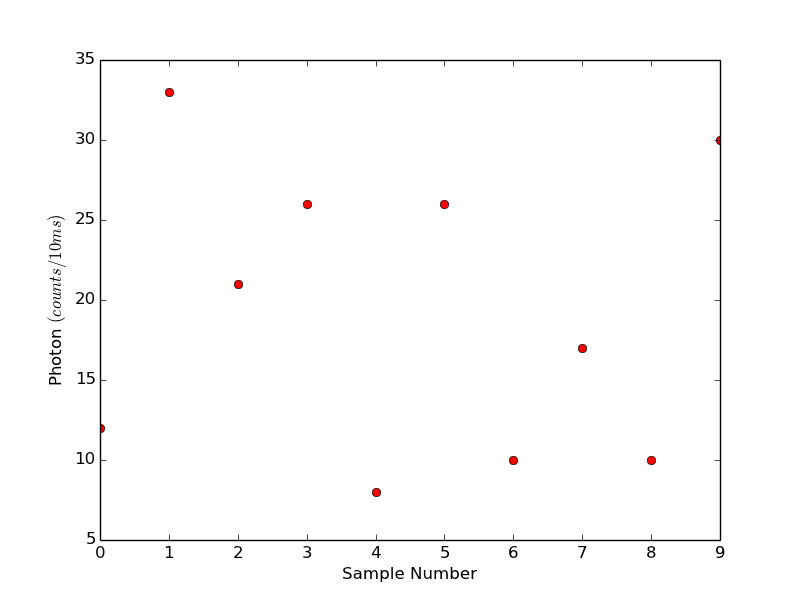
\includegraphics[scale=0.7]{figure_1}
\caption{\small{shows an x-axis of 10 data samples ranging 0-9 and y-axis being the number of photons counted in the 10ms interval. with a {\it mean} = 19 photons, $\sigma$ = 8.68 }}
\end{figure}
\end{center}

\begin{center}
\begin{figure}[!hb]
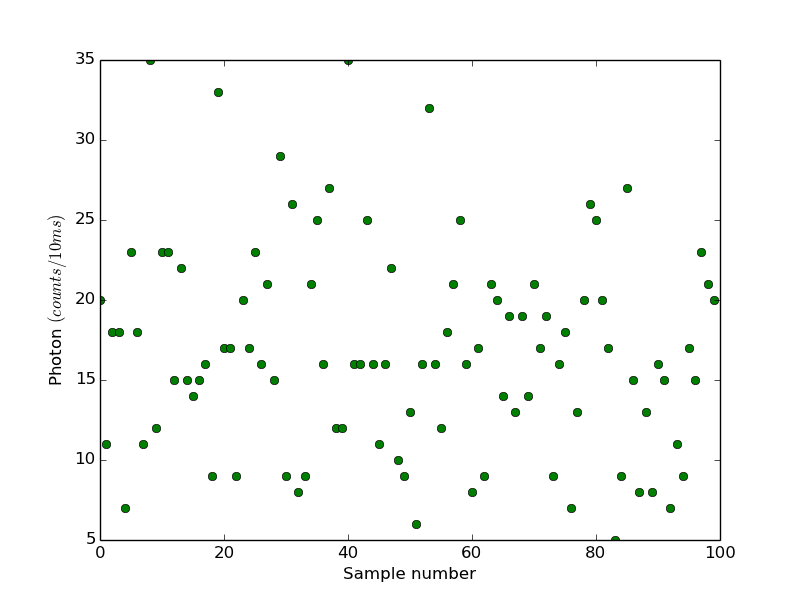
\includegraphics[scale=0.7]{figure_2}
\caption{\small shows an x-axis of 100 data samples ranging from 0-99 and y-axis being the number of photons counted in the 10ms interval. With an increase of data samples we show that the mean and standard deviation $(\sigma)$ decreases: {\it mean} = 16 photons , $\sigma = 6.46$.}
\end{figure}
\end{center}

\begin{center}
\begin{figure}[!hb]
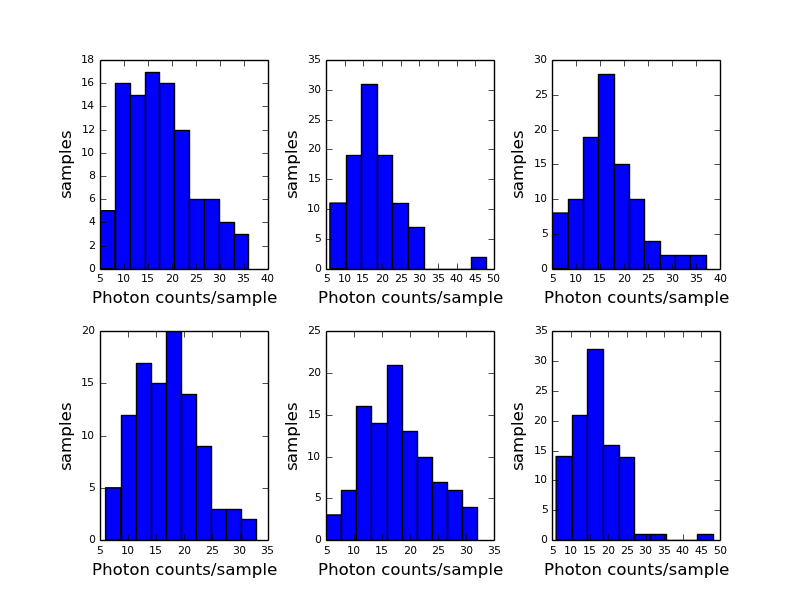
\includegraphics[scale=0.7]{figure_3}
\caption{\small All 6 plots use 1000 samples with 10 ms intervals (graphs 1-3 top right to left | graphs 4-6 bottom left to right). graph 1: mean = 17.80, $\sigma$ =6.74 | graph 2: mean = 17.96 photons, $\sigma$ = 6.89 | graph 3: mean = 16.49, $\sigma$ = 6.04 | graph 4: mean = 17.16, $\sigma$ = 5.57  | graph 5: mean = 17.77, $\sigma$ =5.91 | graph 6: mean = 17.01, $\sigma$ = 6.21 | All data sets combined: mean = 17.37, $\sigma$ = 6.27}
\end{figure}
\end{center}

\begin{center}
\begin{figure}[!hb]
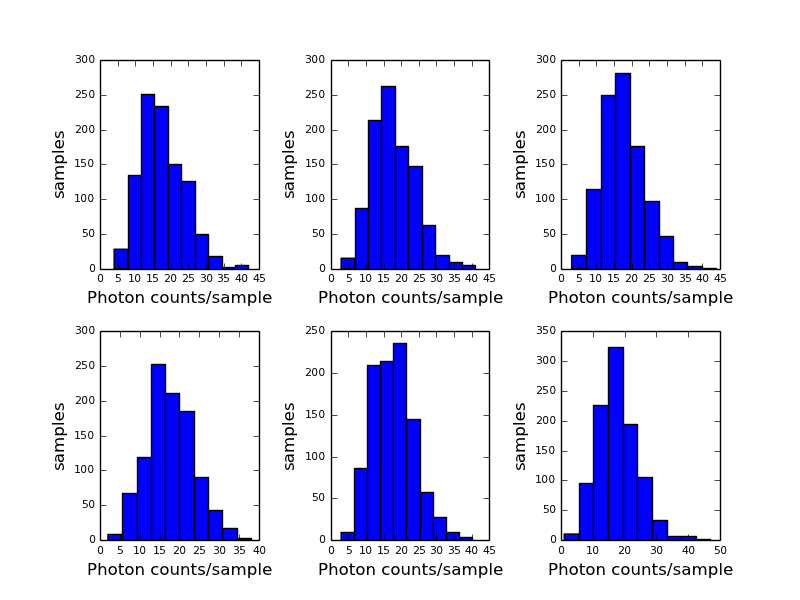
\includegraphics[scale=0.7]{figure_4}
\caption{\small All 6 plots use 1000 samples with 10 ms intervals (graphs 1-3 top right to left | graphs 4-6 bottom left to right). graph 1: mean = 17.54 $\sigma$ =6.10 | graph 2: mean = 17.68 photons, $\sigma$ = 6.03 | graph 3: mean = 17.68, $\sigma$ = 5.82 | graph 4: mean = 17.62, $\sigma$ = 5.83  | graph 5: mean = 17.74, $\sigma$ =5.75 | graph 6: mean = 17.57, $\sigma$ = 6.17 | All data sets combined: mean = 17.64, $\sigma$ = 5.95 }
\end{figure}
\end{center}

\begin{center}
\begin{figure}[!hb]
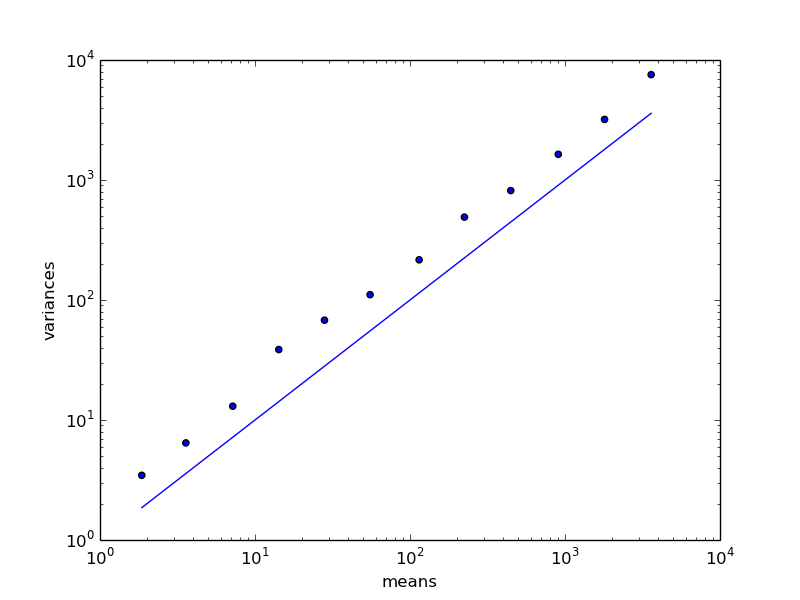
\includegraphics[scale=0.7]{figure_5}
\caption{\small A log scale on both axis variance ($\sigma^2$) vs. means. The points being the collected data and the line being the predicted data. The data has the same slope as the prediction except every value having then same y-value offset from the prediction. }
\end{figure}
\end{center}

\begin{center}
\begin{figure}[!hb]
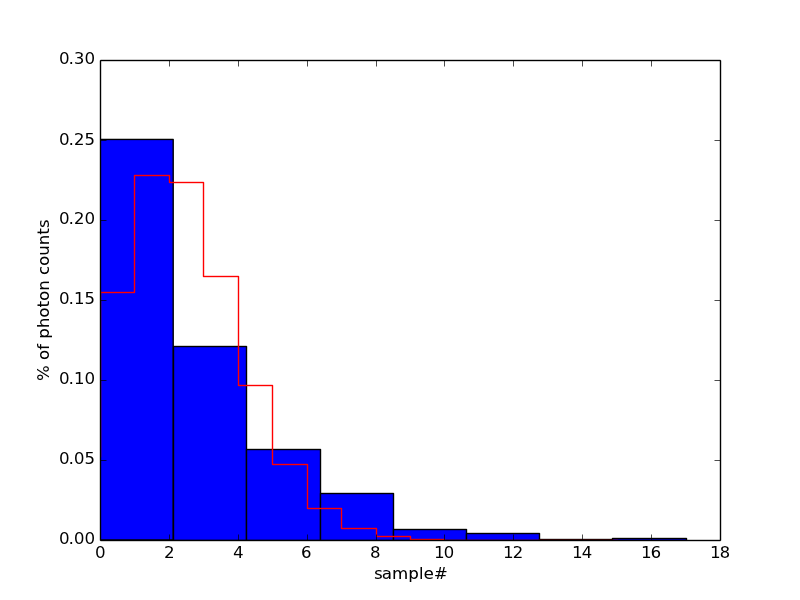
\includegraphics[scale=0.7]{figure_6}
\caption{\small A histogram of blue being the actual values and the red line histogram being the predicted values for a Poisson Distribution. The graph is normalized so the area under both histograms is equal to 1. The Poisson distribution equation p(x,$\mu$) = $\frac{\mu^x}{x!e^\mu}$ where $\mu$ = 2.943 is the mean counts and x =16 is the range value. The mean value of the theoretical Poisson distribution value is P= .062}
\end{figure}
\end{center}

\begin{center}
\begin{figure}[!hb]
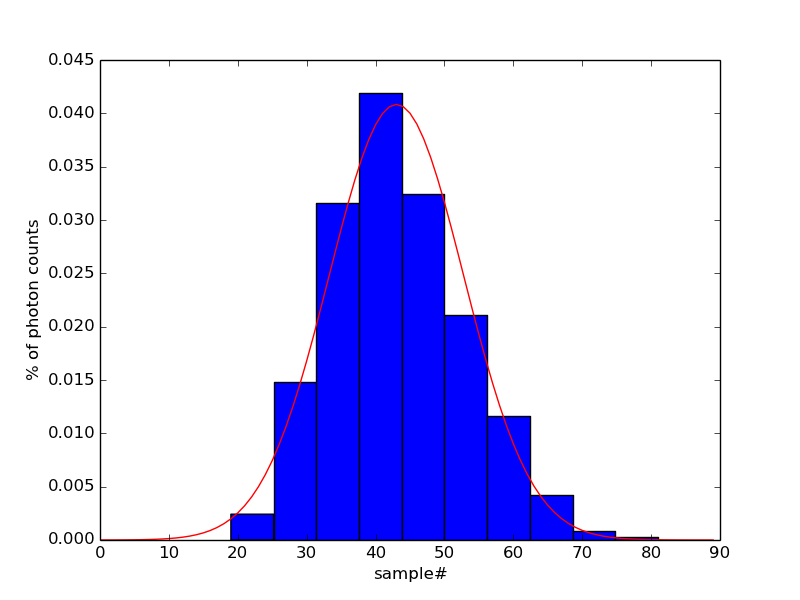
\includegraphics[scale=0.7]{figure_7}
\caption{\small A Gaussian probability distribution: p(x,$\mu,\sigma$) = $\frac{1}{\sigma\sqrt{2\pi)}}*-.5( \frac{x-\mu}{\sigma})^2$ where $\mu$ is the mean counts $\sigma$ is the standard deviation and  x is the range value. In this case the the Poisson distribution is very similar to the Gaussian probability distribution}
\end{figure}
\end{center}

\begin{center}
\begin{figure}[!hb]
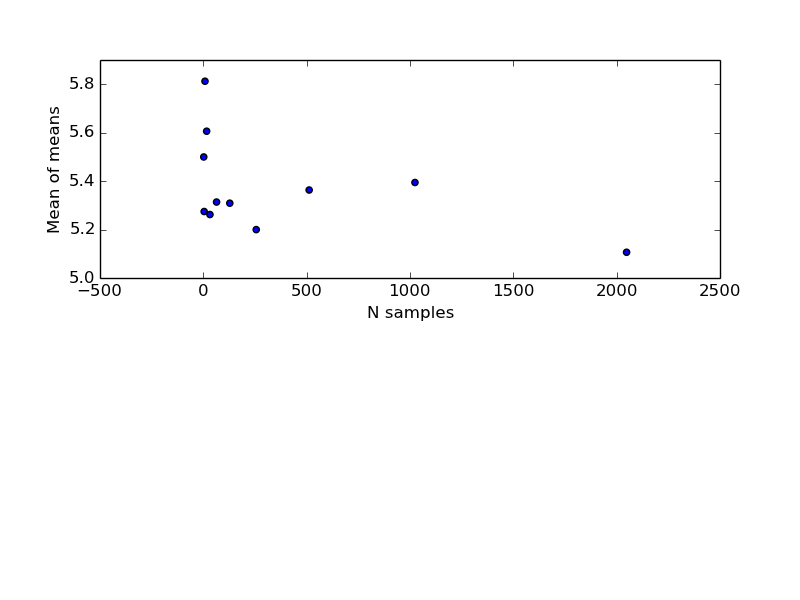
\includegraphics[scale=0.7]{figure_8}
\caption{\small Calculating the mean of means as the number of samples per data set increases exponentially at $2^n$ of n ranging from n=1 to n=11. A large spike at the beginning then a gradual descent of slope is what is  expected when a sample size of 128 and 256 are outliers. }
\end{figure}
\end{center}

\begin{center}
\begin{figure}[!hb]
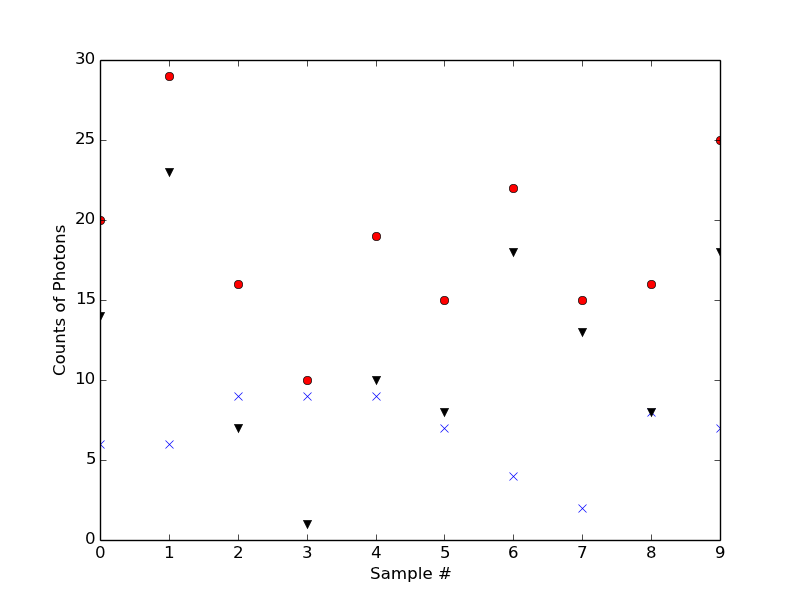
\includegraphics[scale=0.7]{figure_9}
\caption{\small A single data set shows points of when a background LED is ON (red dots) vs. OFF (blue x's)with a second LED at a low brightness setting. Their differences are shown as upside-down triangles.}
\end{figure}
\end{center}

\begin{center}
\begin{figure}[!hb]
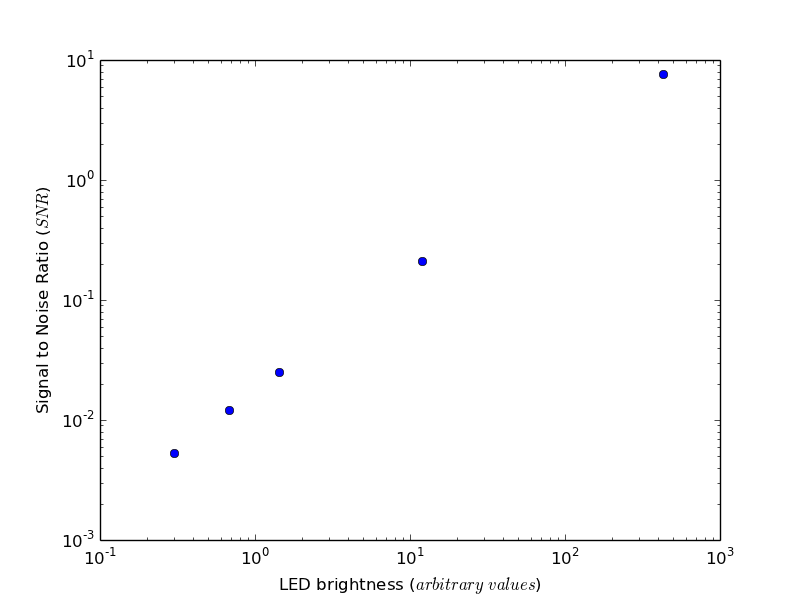
\includegraphics[scale=0.7]{figure_10}
\caption{\small A log scale on both axis with the x-axis as an arbitrary increase in LED brightness. The y-axis shows a signal to nose ratio (SNR) where the background LED is on and the second LED has an increase in brightness while getting rid of the background noise (false positive detection of photon)}
\end{figure}
\end{center}



\end {document}